\section{Experimental setup}
The experimental setup consists of a control unit, the detector unit and a computer with an application for the visualization and data taking. The control unit is connected to the detector unit using a ribbon cable and to the computer via a USB connection. Located on the control and detector unit is a glass fiber connection that is used to point a laser from the control unit onto the detector. Additionally, a strontium-90 source is provided, along with the shielding for its application.

\subsection{Detector unit}
The detector unit mainly consists of the silicon strip detector with 128 strips and a BEETLE readout chip. The silicon strip detector consists of a n doped silicone base with inlayed p doped silicone strips. The strips are then isolated by a $\mathrm{SiO}_2$ layer to which the readout electronics are connected. The thickness of the silicone strip sensor is \qty{300}{\micro\meter}. A schematic diagram of the sensor is shown in \autoref{fig:schematic} and a macroscopic picturfe is given in \autoref{fig:micro} \cite{V15}. 



\begin{figure}[H]
	\centering
	\begin{subfigure}{0.45\textwidth}
		\centering
		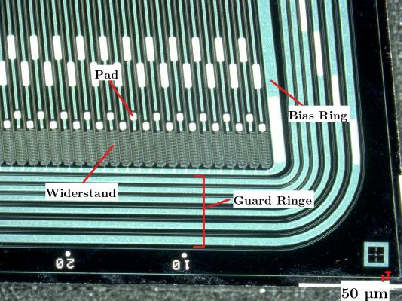
\includegraphics[width=\textwidth]{Assets/micro}
		\caption{Macroscopic picture of the silicone strip sensor \cite{V15}.}
		\label{fig:micro}
	\end{subfigure}
	\hfill
	\begin{subfigure}{0.45\textwidth}
		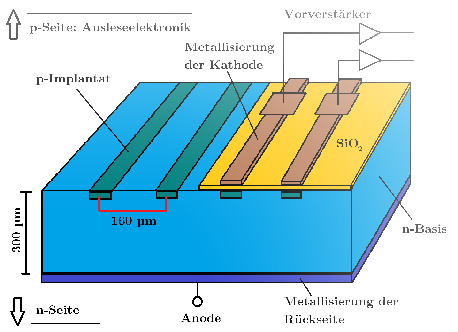
\includegraphics[width=\textwidth]{Assets/schematic}
		\caption{Schematic diagram of the silicone strip sensor\cite{V15}.}
		\label{fig:schematic}
	\end{subfigure}
\end{figure}


In the case of a not fully depleted sensor, some of the electrons and holes generated by the ionizing particles are recombined outside of the depletion zone. The charge collection efficiency (CCE) describing this process when applying a laser is given by 

\begin{equation}
	\mathrm{CCE}(U)=\frac{1-\exp\left(\frac{-d_{\mathrm{c}}(U)}{a}\right)}{1-\exp\left(\frac{-D}{a}\right)},
	\label{eq:charge_col_eff}
\end{equation}
where $a$ is the penetration depth of the laser.

\subsection{Laser}
The Laser employed in this experiment is fed into the detector unit using an optic fiber cable. It has a wavelength of \qty{980}{\nano\meter}, a diameter of \qty{20}{\micro\meter}, a pulse length of \qty{5}{\nano\second}, and a peak power of \qty{0.2}{\milli\watt}. The position and the focusing of the laser can be adjusted using two micrometer screws.
\subsection{Control unit}
The control unit houses the laser and is used to regulate the voltage applied to the silicone sensor. It can also measure the leakage current of the sensor. The data acquired by the control unit is transferred to the computer and can be collected there using the Alibava system.

\section{Experimental procedures}
\label{sec:exec}
Before starting the experiment, it is advisable to become familiar with the experimental setup and the software. In the initial measurement, the current passing through the sensor is recorded at intervals of \qty{10}{\volt} for the applied voltages. This is performed until a voltage of \qty{20}{\volt} above the expected depletion voltage is reached.\\

The first measurement using the software is performed in a \textit{pedestal run} of 1\,000 events, in order to determine the pedestal and the noise.\\

Before using the laser or the radioactive source, a set of calibration measurements are started. The first calibration is used to determine the optimal delay. It is started using the \textit{Delay measurement} button in the Alibava software. After this run, five different channels are used in a \textit{Calibration run}, with the applied voltage above the depletion voltage. Another run is started afterwards with the applied voltage turned down to \qty{0}{\volt}.\\

After the calibration measurement, the laser is lead into the detector unit using the optic fiber cable. It is then focused and moved along the sensor until a maximally high peak is achieved in the Alibava software. Initially the optimal delay between the laser signal and the chip readout is determined using the \textit{laser sync.} function. Then the structure of the sensor is probed by recording 1\,000 events at 35 \qty{10}{\micro\meter} intervals. During the next measurements the CCE is determined by recording 1\,000 events from 0 to \qty{200}{\volt} in \qty{10}{\volt} steps.\\

A similar approach is used when measuring the radioactive source, with the difference of recording 10\,000 events per scan. \\

Finally a last scan using the radioactive source is performed and 1\,000\,000 events are recorded.